\documentclass[14pt,fleqn]{extarticle}
\RequirePackage{prepwell-eng}

\previewoff

\begin{document} 

\begin{skill}
    \begin{narrow}
\textcolor{blue}{Parabola Basics }         
    \end{narrow}
    
    \reason 
    
    \begin{center}
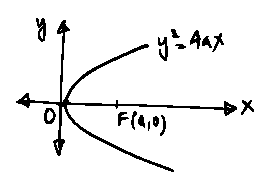
\includegraphics[scale=1.2]{parabola.eps} 
\end{center} 

\begin{center}
  \begin{tabular}{Nl}
  \toprule 
  & \bf{Definition} \\
  & The locus of all points that are equi-distant\\
  & from a line (called \textit{directrix}) and a point \\
  & (called the \textit{focus}) \\
  \midrule 
        &  \bf{In the figure above} \\
   \midrule 
   1 & $F$ is the focus. The directrix \\ 
   & has not been shown  \\ 
   \midrule 
   2 & $F$ always lies on the axis of \\
   & the parabola \\ 
   \midrule 
   3 & The vertex is where the parabola \\
   & cuts it's axis (point $O$) \\ 
    \midrule 
   & \bf{You will only study parabola $\ldots$} \\
   A & With focus $F$ on the $x-$ or $y-$ axis only \\
   \midrule 
   B & Vertex at the origin only \\
    \bottomrule
  \end{tabular}
\end{center}


\textbf{Standard equations} 
\begin{center}
  \begin{tabular}{cN}
  \toprule 
        Opens along & \text{Standard Equation}  \\
   \midrule 
   Positive $x$ axis & y^2 = 4ax \\
    \midrule 
    Negative $x$ axis & y^2 = -4ax \\ 
    \midrule 
    Positive $y$ axis & x^2 = 4ay \\ 
    \midrule 
    Negative $y$ axis & x^2 = -4ay \\
    \bottomrule
  \end{tabular}
\end{center}
    
\end{skill}
\end{document} 